\section{Results}

\subsection{Data sets}
We used synthetic data set of \cite{rampasek2014fcnv} based on sequencing data of mother-father-child trio I1 published by \cite{kitzman2012}. This data set consists of 360 CNV cases simulated \textit{in silico} in chromosome 1 of I1 maternal plasma sample. These 360 cases fall into 36 categories defined by 6 different CNV types (maternal/paternal deletion, maternal/paternal duplication of haplotype A/B) and 6 different CNV lengths, with 10 cases for each of these ``type $\times$ length'' categories. We randomly split this data set to a training set of 300 cases and a testing set of 60 cases, while maintaining the relative abundance of the 6 different CNV types constant across both sets. That means the training and testing sets are mutually unbiased towards CNV types.

\subsection{Model training}
We trained 4 sets of feature weights by one randomized pass over the training set. For each training method (gradient and maximum margin training) we trained 2 models -- with, and without copy count priors (depth-of-coverage information), respectively. As the initial weights for edge features (in each distance bin) we chose the log of transition probabilities used in the HMM by \cite{rampasek2014fcnv}. Note that there is no difference between edge features' weights between different distance bins in this initialization. The beta-binomial and copy count prior feature weights were both initialized to 1.

\subsection{CRF performance}
\begin{figure*}
\caption{Performance of our CRF before training with initial weights corresponding to logarithm of transition probabilities of the HMM. Results are presented for model with and also without copy count prior, respectively.}
\label{fig:CRFinit}
\centering
\hspace*{-8pt}
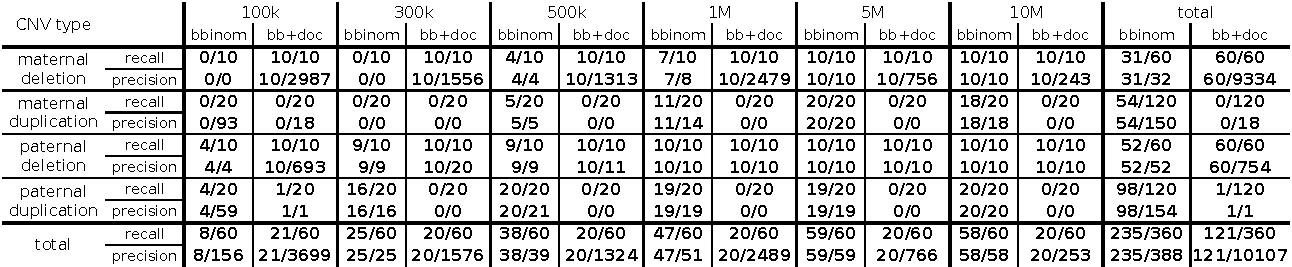
\includegraphics[width=1.03\textwidth]{figures/crf_initial_all}
\end{figure*}
First, we tested our CRF model with the initial parameters. The results on all of the data set combined are presented in Figure \ref{fig:CRFinit}. CRF without the depth-of-coverage feature, but with these initial parameters, conceptually corresponds to the original HMM. As the results show, this is a very good initialization of the edge feature weights. When we included also the depth-of-coverage feature, we see a significant performance drop, this is because weights for both node features (beta-binomial model and DOC-based prior, respectively) have the same weight. Their relative importance for correct CNV prediction needs to be learnt from the data.


The obtained results on training and testing set are shown in Figure \ref{fig:CRFresAll}. Our training did not work as expected as the model almost never calls any CNVs.

\begin{figure*}
\caption{Performance of our CRF with different sets of feature weights. Results are presented on both training and testing set, respectively.}
\label{fig:CRFresAll}
\centering
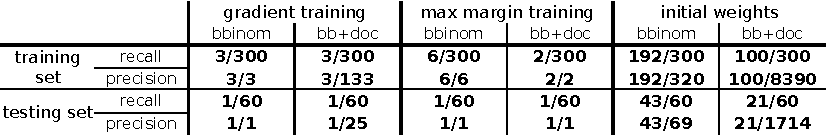
\includegraphics[width=0.7\textwidth]{figures/crf_res_all}
\end{figure*}

%In the Figure \ref{fig:CRFinit} we show CRF performance with initial set of weights without any sort of training. Further, Figures \ref{fig:CRFbyGM} and \ref{fig:CRFbyMM} show performance of our CRF after training by gradient and maximum margin method, respectively.
%
%\begin{figure*}
%\caption{Performance of our CRF before training with initial weights corresponding to logarithm of transition probabilities of the HMM. Results are presented for model with and also without copy count prior, respectively.}
%\label{fig:CRFinit}
%\centering
%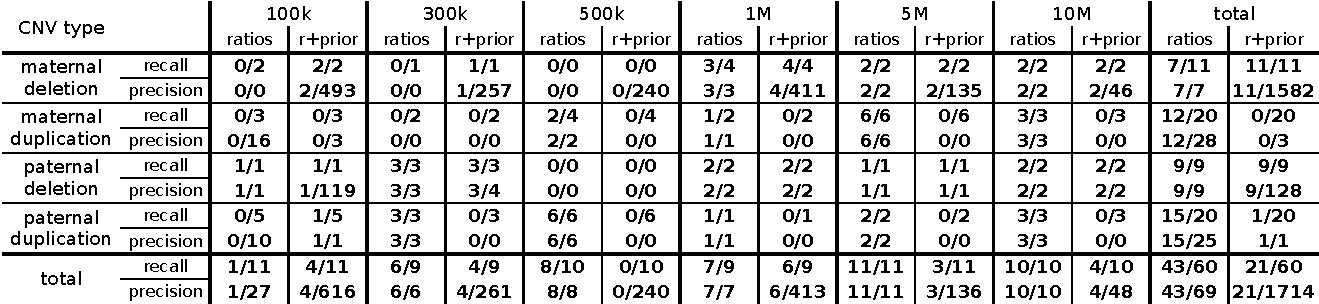
\includegraphics[width=0.99\textwidth]{figures/crf_initial_w}
%\end{figure*}
%
%\begin{figure*}
%\caption{Performance of our CRF trained by gradient method with and without copy count prior, respectively.}
%\label{fig:CRFbyGM}
%\centering
%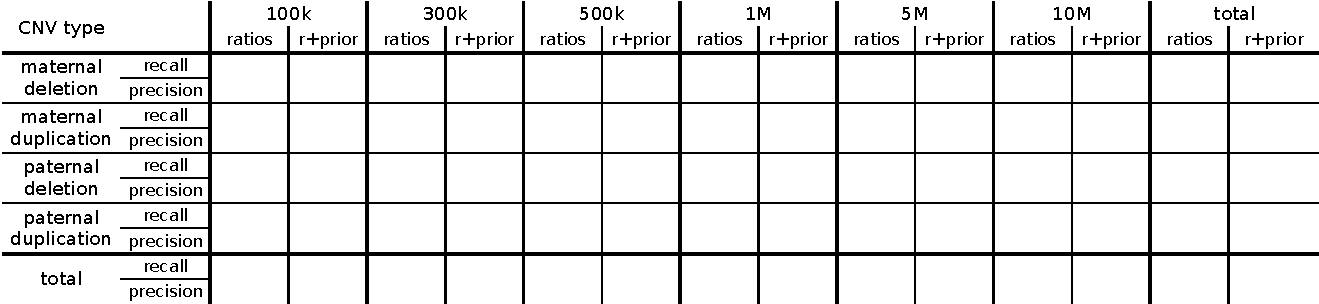
\includegraphics[width=0.99\textwidth]{figures/crf_gradient}
%\end{figure*}
%
%\begin{figure*}
%\caption{Performance of our CRF trained by maximum margin method with and without copy count prior, respectively.}
%\label{fig:CRFbyMM}
%\centering
%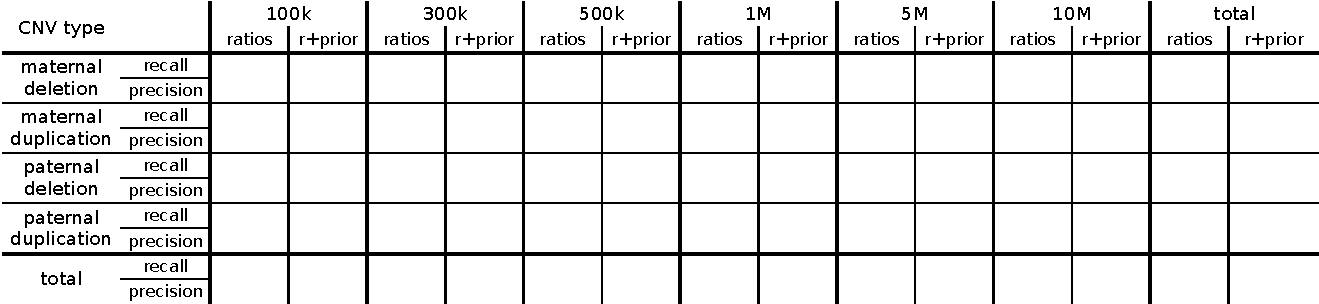
\includegraphics[width=0.99\textwidth]{figures/crf_margin}
%\end{figure*}

\subsection{Beta-binomial model vs. multivariate Gaussian model in HMM framework}
\begin{figure*}
\caption{Performance of beta-binomial vs multivariate Gaussian allele counts model in the original HMM framework}
\label{fig:BBvsMG}
\centering
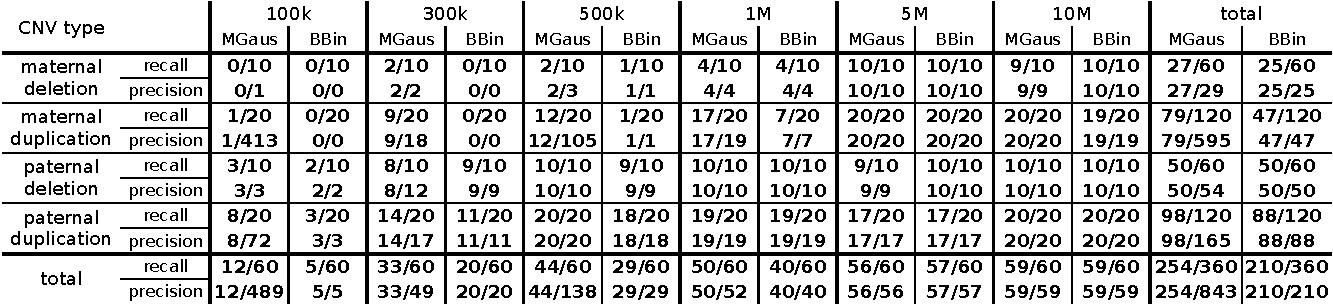
\includegraphics[width=0.99\textwidth]{figures/hmm_bb_mg}
\end{figure*}
To evaluate the performance influence of the beta-binomial model on the performance of our model, we compared performance of the HMM as described in \cite{rampasek2014fcnv} with the original multivariate Gaussian model and with beta-binomial model for allele distribution, respectively. We did not include the copy count priors in the models for these experiments, i.e. only the allelic counts signal was used. The results are in Figure \ref{fig:BBvsMG}. The results suggests that the beta-binomial model is a significantly more precise model, however with decreased sensitivity.


%\subsection{Project goals}
%More concretely, the goals of this project are:
%
%\begin{enumerate}
%
%\item Test CRF models by trying different features (including DOC and allelic ratios) and exploring training procedures in the simulated training set regime. Training may include initializing the CRF with the converted HMM conditional distribution features and weights and fine-tuning with the discriminative objective. Training algorithms worth exploring are maximum likelihood training with L-BFGS or an online large-margin procedure as in \cite{bernal2007}.
%
%\item (optional) Model parental CNV as called by CNVnator on the respective WG sequencing samples. Explicitly pre-computing and utilizing information about these potentially inherited CNVs is likely to reduce the false positive rate.
%
%\item (optional, more challenging) Investigate how to extend the method to eliminate the need for explicit knowledge of paternal genotype. This is an important issue for potential clinical use, not only for the implied cost reduction, but mainly because paternal genotype might be difficult or impossible to obtain in practice.
%
%\end{enumerate}
%While goals (2) and (3) are important for clinical practise, we plan to focus our efforts mainly on the machine learning aspects as described in (1).


%%%%%%%%%%%%%%%%%% FIGURE TEMPLATES %%%%%%%%%%%%%%%%%
%%%%%%%%% SINGLE FIGURE %%%%%%%%
%\begin{figure}
%\caption{caption fdfd}
%\label{fig:}
%\centering
%\includegraphics[height=0.33\textheight]{figures/}
%\end{figure}
%
%%%%%$%%%% MULTIFIGURE %%%%%%%%%
%\begin{figure*}
%\caption{caption fdfd}
%\label{fig:}
%\subfigure[subfig title A]{ 
%\begin{minipage}[b]{0.48\textwidth}
%	\centering
%	\includegraphics[width=0.98\textwidth]{figures/}
%	\end{minipage}	
%}
%\subfigure[subfig title B]{
%	\begin{minipage}[b]{0.48\textwidth}
%		\centering
%	\includegraphics[width=0.98\textwidth]{figures/}
%	\end{minipage}	
%}
%\end{figure*}
